%!TeX spellcheck = en-US
\documentclass[../main.tex]{subfiles}
\begin{document}

\chapter{Testing and Validation}

\label{chap:fuzzing}

\section{Software testing}

Software testing can be conceptually divided into two main groups: \textbf{Static Testing} and \textbf{Dynamic Testing}. While \textbf{Static Testing} is based on a (human) review of the source code, without executing the program, the \textbf{Dynamic Testing} is mainly accomplished with the use of automated tools at run time. In particular, many different tests can be conducted on a single piece of software by an autonomous program. The results of such tests are then used to correct bugs in production (e.g. agile development) or to exploit such bugs if the test is conducted by a malicious counterpart.

The research was carried out mainly using \textbf{Dynamic Testing} and in particular Fuzz testing mixed with other methods such as source code review and reverse engineering. A \textbf{Dynamic Test} can be of three types: \textbf{Black Box}, \textbf{White Box} and \textbf{Gray Box} depending on the level of knowledge and access to the source code required.

\subsection{Black Box}

For this methodology no access to the source code or knowledge of the design
specifications and internal mechanisms of the program is required. The test is
based only on what can be observed, which means to give the target different
inputs and monitor its behavior. This definition reflects exactly the
interaction that a typical user might have with the program. Which are exactly
the cases that this kind of testing wants to examine and it should test typical
and atypical user behavior. Black Box testing is widely used and it includes all
the techniques where the only available information comes from the user
interaction with the application. One example among all is SQL injection, where
the test is conducted against a plain web page without any previous knowledge of
the logic of the servers and the various scripts. Only interacting with them
allows the user to get an idea of the inner working mechanisms. The test can be
performed directly by the user (manual testing) or using ad hoc programs
(automated testing) such as SQLmap\footnote{\url{http://sqlmap.org/}} in this case.
Black Box testing has many advantages: mainly, it does not require access to the
source code so it is always applicable; moreover, even in the presence of source
code, it can still be effective. In addition to this, since it is not source code dependent, a successful test case against one program (for example a zip extractor) can be easily reused to test any programs that implement the same functionality.

However, due to its simplicity this approach can only scratch the surface of the
application that is being tested, achieving an extremely low code coverage. Moreover complex vulnerabilities, which requires multiple attack vectors, will never be triggered and can only be discovered with a White Box or static approach.

\subsection{White Box}

This methodology is nothing more than a source code review or analysis and it
can be done either by a human being or, more often, by automated tools. Human
analysis in not always feasible and might be inaccurate, especially in large
projects, because it is easy to miss one line or make simple mistakes. For this
reasons automated source code analysis is the means used in a White Box approach. This method has many advantages mainly regarding code coverage since it is possible to test all the paths for vulnerabilities. However, source code is rarely available for projects outside the open source community and this approach still requires a human interaction to review the results and identify the parts that are actually related to security problems. Moreover, reviewing a large project, even with the use of automated tools, might require significant time to complete, effectively bringing the performance down to the level of the Black Box approach.

\subsection{Gray Box}

The definition of this technique is quite trivial because several different
methods can be seen as Gray Box approach. This takes the Black Box method as a
starting point augmenting it with the use of common reverse engineering and
binary analysis techniques using disassemblers, debuggers and similar tools. The
majority of these tools still requires human interaction and, reverse
engineering a program can often be a tedious and hard job. However, there are
some automated tools that aim to facilitate this analysis, such as Ropper\footnote{\url{https://scoding.de/ropper/} - \url{https://github.com/sashs/Ropper}} which provides
information about a binary and automatically searches for particular
vulnerabilities (ROP and JOP) or Frida\footnote{\url{https://www.frida.re} - \url{https://github.com/frida/frida}} which allows the user to inject snippets of code inside a Black Box binary. For these reasons the Gray Box technique can efficiently improve the coverage produced by the classic Black Box approach still without requiring access to the source code. Moreover this approach becomes very powerful if the source code is available as it can modify the program during the compilation phase to efficiently trace the execution flow and the internal state. The information gathered with this method can then be used directly by the user or by another program to better conduct further tests.

\section{The fuzzing world}

\textit{"Fuzzing is the process of sending intentionally invalid data to a
product in the hopes of triggering an error condition or fault."}
\cite{Sutton2007}

Fuzz Testing dates back to 1989 when it started as a project of the Operating
Systems course at the University of Wisconsin-Madison. At his first stages it
was nothing more than a simple Black Box technique to test the robustness of
some UNIX utilities. The first two fuzzers \textit{fuzz} and \textit{ptyjig},
developed by two students, where incredibly successful in finding previously
unknown vulnerabilities: they where able to crash around 30\% of the considered
utilities using random inputs~\cite{firstFuzzPaper}.
It quickly became clear that this was a powerful and strong technique to test
the robustness of a piece of software.

During the years fuzz testing evolved and developed gaining popularity and
expanding to more and more fields (networks, files, wireless and more) until it
became a proper domain of research and engineering. As for today it is
quite vast and, using this kind of tools in the software testing phase would be the best practice. Nevertheless it is still uncommon to find fuzzing
outside the security world, so it is hard to give a precise and unique
definition for this technique. I will try to give an overview of the actual fuzzing world focusing mainly on the binary fuzzing and explaining how the previously mentioned techniques are applied to the fuzzing field.

Fuzzers can be at first divided into two main categories:

\begin{itemize}
  \item{\textbf{Mutation Based (or Dumb)}: it applies random mutations to the
  given  input without any knowledge of the data that are being manipulated.
  Common  mutations include bitflipping, shortening or expanding the input and
  similar.  This  method is a really simple and pure brute force approach and it
  can be  applied  to user provided inputs as well as to automatically generated
  ones to  progressively create a valid input.}

  \item{\textbf{Generation Based (or Smart)}: it requires some knowledge of the
  data or protocol that is being fuzzed and this information is then used to
  generate proper inputs. Such information is either provided by the user
  who defines a specific set of rules or autonomously extracted from a sample
  by the  fuzzer and can be used to generate valid CRC codes for mutated  strings  or  keep the correct  structure for particular files (jpg). Obviously this approach has some  advantages but in some cases a mutation based approach can  give better results  as it can test programs even outside their functioning  boundaries.}

\end{itemize}

Predictably a fuzzer that combines the two methods is the one that can give the most comprehensive results.

Fuzzers can be associated with the previously mentioned testing methods. In this way fuzzers can be further differentiated based on the approach that they have to the problem and the information they require to test the binary. This divides the fuzzing world in three theoretical categories: \textbf{BlackBox Fuzzing}, \textbf{WhiteBox Fuzzing} and \textbf{GrayBox Fuzzing}. \textbf{BlackBox Fuzzing} is the pure Black Box approach, discussed earlier. It can be both mutation and generation based and it can usually only scratch the surface of a program as its behavior is based only on the output produced by the tested program. Therefore it is unlikely that this method will produce a test case able to deeply explore all the code and, for example, trigger nested if conditions. \textbf{WhiteBox Fuzzing} requires access to the source code and is a really sophisticated approach which is rarely used since it uses code analysis to generate test cases that will produce full code coverage. For this reason this approach is usually resource and time intensive. \textbf{GrayBox Fuzzing} is halfway between the two and it usually works with or without access to the source code. This method consists in injecting special code during the compilation phase or sandboxing the binary inside an emulator in order to extract information on the execution status and the code coverage achieved. With knowledge on the internal status it is also easier to test the program for particular conditions or specific cases.

However, fuzzing is not an exact science and in the real world choosing the right approach can be trivial and usually there is not a clear distinction between the different categories.


\section{State of the art}

There is much software available for many different fuzzing jobs. The choice is vast and goes from the simple hobby project to the much more complex and advanced commercial software. Choosing a good fuzzer is a crucial step for the success of the task: a fuzzer, which is too basic and relays solely on a pure brute force approach (like \textit{ptyjig}) can require ages to find a simple bug on a modern program, whereas a "smarter" fuzzer, will take just a few minutes or hours.

This section is focused on binary fuzzers since the main objective of this research is to test binary tools.
\acrlong{afl}, which was used in this research as it offers many features and it is extensively documented, and Peach represent the actual state of the art in term of binary fuzzers.

In the following two sections there is an overview of this two tools.

\subsection{American Fuzzy Lop}

\acrlong{afl} or \textbf{\acrshort{afl}} \footnote{\url{http://lcamtuf.coredump.cx/afl/}} represents the state of the art among binary fuzzers and it has a high rate of vulnerability discovery as stated in the "bug-o-rama trophy case" section of the website. Moreover it is widely used and in active development.

\textbf{\acrshort{afl}} has many different features that makes it a quite sophisticated software. It is mainly based on a Gray Box approach, which require access to the source code in order to perform what it calls "instrumentation". This process consists in adding some custom code to the program that is being compiled; this automatic operation, performed by the dedicated compilers \textit{afl-gcc} and \textit{afl-clang-fast}, adds small code snippets in critical positions without weighing down the program but allowing the fuzzer to obtain information on the execution flow at run time. It also uses a \textbf{Mutation Based} approach which relies on  some statistical methods to optimize the generation making it efficient and fast to setup.

In addition to instrumentation, \textbf{\acrshort{afl}} can fuzz Black Box binaries leveraging the QEMU emulator to obtain information about the execution state of the binary and adjust the generation method accordingly. Adopting a Black Box approach can be useful also when the source code is available since it can highlight vulnerabilities introduced in the compilation/optimization phase. However this can result in reducing the execution speed which considerably slows down the testing.

The information gathered by the fuzzer at execution time will then be used to meaningfully mutate the input. \textbf{AFL} has two different input generation strategies depending on the information supplied: if a file containing a valid input for the program is provided, it is used as a starting point to the next stages. Otherwise, if a blank file is supplied, \textbf{AFL} starts a "0-day" input generation. This last technique has been proven to be particularly successful, even if more time consuming than the other one. Interestingly it enabled \textbf{AFL} to generate valid URLs, JPG headers, XML syntax and more~\cite{aflblog}. More specifically the fuzzer uses a genetic algorithm approach which keeps a queue of interesting inputs that will then be mutated. It will append a file to the queue if it triggers a previously unknown internal state. Three different deterministic mutation strategies are applied:
\begin{enumerate}
  \item \textit{Sequential bitflips with varying lengths and stepovers}: this is a slow but very effective way of mutating the input as it has been observed that, with different length of bitflipping, it is possible to generate around 130 new paths per million input.
  \item \textit{Sequential addition and subtraction of small integers}: this method consists in incrementing or decrementing existing integer values in the input file. The operation is performed in 3 different stages: firstly on 8-bit values, then on 16-bit values and lastly on 32-bit values all in both endianess. These last two methods are performed only if during the operation the most significant byte is changed; otherwise the value has already been tested in one of the previous cases.
  \item \textit{Sequential insertion of known interesting integers}: this method uses particular values that are known for their ability to trigger interesting cases, for example $-1, MAX\_INT, MAX\_INT-1$ and so on. The values are tested in both endianess and in 8,16,32 bits representation.
\end{enumerate}

There are also non deterministic strategies applied in a never ending loop which include insertions, deletions, arithmetic, and splicing of different test cases \cite{afltech}.

Moreover \textbf{AFL} can be parallelized on many cores, in this way there will be a Master process that coordinates other Slave processes. All the orchestration and synchronization of the processes is handled automatically by \textbf{AFL}. The Master process will perform all the deterministic mutations while the Slaves will perform the random mutations, since the random mutations are faster to perform the Slaves will progress faster than the Master greatly speeding up the testing. In addition to this the fuzzer is also able to resume previously interrupted jobs without losing the progresses and the found crashing inputs.

\textbf{AFL} comes with a very informative user interface as it can be seen in Figure \ref{fig:aflint}.

\begin{figure}[htp]
  \centering
  \hspace*{0.6cm}
  \vspace*{0.6cm}
  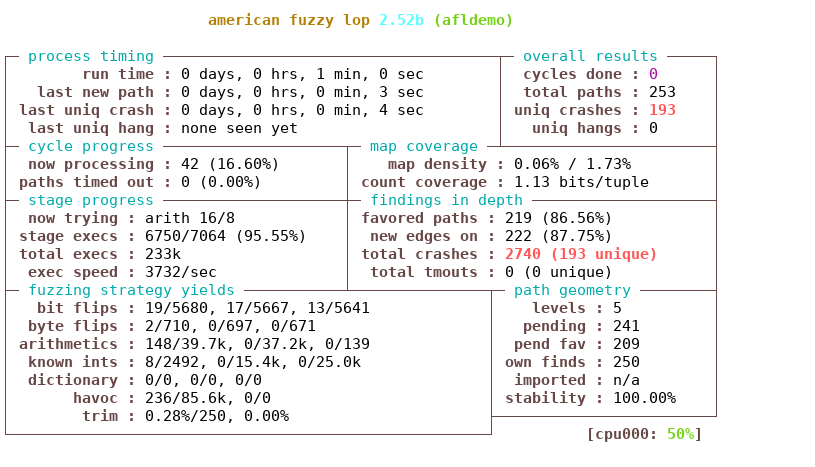
\includegraphics[scale=0.7]{images/afl-test_x86_64-white.png}
  \caption{AFL interface}
  \label{fig:aflint}
\end{figure}

The most interesting and relevant parts are described here:

\begin{itemize}
  \item \textit{Overall Results}. The first field in this section shows the count of queue cycles done so far. This is the number of times the fuzzer consumed all the interesting test cases in the queue, fuzzing them, and started over from the very beginning.

  \item \textit{Map Coverage}. This section gives insights about the results of the instrumentation and the internal state of the program. The first line shows how many branch tuples have already been hit, in proportion to how many are expected for this binary; this value is stored in a bitmap file. The number on the left describes the current input and the one on the right is the value for the entire input corpus.

  The second line shows the hit counts for the branch tuples of the binary. If every branch is taken for a fixed number of times for all the inputs, this value will be  $1.00$. As other hit counts are triggered for every branch the value will move towards $8.00$ (every bit in the 8-bit map hit).

  \item \textit{Stage Progress}. This section gives an image of what the fuzzer is actually doing. The first line indicates the strategy that is being applied to mutate the inputs. The following two lines show the number of executions for the current stage of the fuzzing and for the entire test procedure. The last line shows the current execution speed of the target to give an idea of the performance of the binary.

  \item \textit{Path Geometry}. This section gives an overview of the inputs generation and discovery. The first line is the "path depth": user supplied inputs are of level 1, then the inputs derived from this are of level 2 and so on following this logic. The second line is the number of inputs not used yet for testing, the third line is the number of entries that are considered really promising by the fuzzer and will be tested in this cycle. Then the other two lines are the number of discovered new paths and of paths imported from other fuzzers during parallelized jobs. At the end, the last line measures the consistency of observed traces: if a program always behaves the same for the same input data, this value will be of 100\%. A too low value indicates that \textbf{AFL} will have difficulty discerning between meaningful and "phantom" effects of tweaking the input file.

\end{itemize}

\bigskip One of the best features of \textbf{\acrshort{afl}} is that it is an open source, meaning that every person can improve the code and modify it to meet different needs. For example one really active researcher in the fuzzing field, Dr. Marcel B\"ohme\footnote{\url{https://comp.nus.edu.sg/~mboehme/}}, created some interesting forks of \textbf{\acrshort{afl}} trying to achieve better code coverage~\cite{aflfast, greybf} and better path discovery~\cite{pythia}.

\subsubsection{afl-unicorn}
\label{sub:afl-unicorn}

\textit{afl-unicorn} is a fork of \textbf{\acrshort{afl}}  that was built to leverage the power of \textbf{\acrshort{afl}} to fuzz trivial binaries.

\textit{"For example, maybe you want to fuzz a embedded system that receives input via RF and isn’t easily debugged. Maybe the code you’re interested in is buried deep within a complex, slow program that you can’t easily fuzz through any traditional tools."}\cite{aflunicorn}.

In particular it uses the Unicorn Engine~\cite{unicorn}, which is a CPU emulator, to run a program using the extracted context from an instance of the same application making it architecture independent and easy to selectively fuzz. As a matter of fact the emulator supports a wide range of CPUs: ARM, AArch64, M68K, Mips, Sparc and X86 thus permitting to easy leverage a different platform for the tests and to directly interact with the virtual processor at execution time. The Unicorn Engine allows to fuzz a program in the exact same way as before but, in addition to this, the user has now control over the memory, the CPU registers and the code of the program. This is useful in many different situations, for example when there is no access to the source code or when the sources are available but it can be more interesting to fuzz a precompiled version of the binary for many different reasons (to test the behavior of a compiler, to test a specific version for a specific architecture and so on). Moreover \textit{afl-unicorn} allows the user to specify portions of code to be fuzzed, i.e. a single function. In addition to this the fuzzing takes place directly inside the emulated memory manipulating a user defined region. It is also possible to write custom "hooks" when certain functions are called or particular addresses are reached so as to skip specific portions of code or to trigger a defined behavior, such as a crash, if the program reaches a defined location in the code.

While it is true that this approach is very powerful it requires a template  to be hand written for the Unicorn Engine. This requires specific information like the heap addresses, the register values and the content as well as the addresses of all the memory regions. The extraction of such information is a trivial process since a binary must be running inside a debugger and, usually, the relevant portion of code must be identified. Only then the template for the emulator can be written. This process is time consuming and requires very specific knowledge of the hardware. As a matter of fact the context of the process must be dumped from the memory and, at the same time, the binary must be disassembled to find the boundaries inside which the emulation must take place.

For those tasks some tools like \textit{unicorn\_dumper.py} and a basic template are provided with the tool; other programs like \textit{unicorn\_template\_generator.py} and \textit{extract\_from\_memory.py} have been written specifically for this task and will be illustrated in Chapter \ref{chap:experimsetup}.

\subsection{Peach}

\textbf{Peach} is another very popular fuzzer and is the commercial counterpart of \textbf{AFL}. However, the two programs are different since \textbf{Peach} is capable of fuzzing different targets such as network protocols, device drivers, file consumers, embedded devices, external devices natively, while in \textbf{AFL} all these capabilities are added by specific forks. Another difference comes in the generation of inputs. As a matter of fact \textbf{Peach} is a \textbf{BlackBox} and \textbf{Generation Based} fuzzer that requires no access to the source code but, instead, a \textit{"Peach Pit"} must be supplied. A \textit{Pit} is a template, defined by the user, that the fuzzer uses to generate the input data, monitor the target and display the status and results. It contains the following information:

\begin{itemize}
  \item A description of the data layout to test.
  \item The agent, monitors and I/O adapter to use in the fuzzing session.
  \item Setup parameters, such as Port or Log Folder, to use in the fuzzing session.
\end{itemize}

As an added factor \textit{Pits} are open source and shared inside the \textbf{Peach} community which makes finding the perfect \textit{Peach Pit} most likely. Moreover from the Whitepaper it is possible to understand that there are \textit{"over 50 mutation algorithms"} but there is no explanation on what these algorithms are doing or how~\cite{peach}.

Peach was open source but from version 3 the policy changed as it is stated on the website: \textit{"Peach is not open source software, it’s FREE software. Peach is licensed under the MIT License which places no limitations on it’s use. This software license was selected to guarantee that companies and individuals do not have to worry about license tainting issues."}~\cite{peachlicense}. This license is ambiguous because on the company website a Community Edition of \textbf{Peach 3} is available and it is stated to be open source (source code is also available). This is probably due to the fact that the company sells fuzzing services using \textbf{Peach} so the commercial version might have more features. However an in development fork of \textbf{Peach 2.7} is maintained by Mozilla.\footnote{\url{https://github.com/MozillaSecurity/peach}}

\end{document}
